%% Los margenes, tipo de hoja y estilo BOOK
\documentclass[a4paper,11pt,twoside,openright,titlepage]{book}
\usepackage[a4paper,left=1in,right=1in,top=0.6in]{geometry}

\usepackage[T1]{fontenc}    %Ineterprete de t�ldes
%\usepackage[utf8]{inputenc}
\usepackage{amsmath,amssymb}    %Paquete de entornos matematicos

\usepackage{natbib}
\usepackage[english,spanish]{babel}
\selectlanguage{spanish} 
\usepackage{graphicx}
\usepackage{psfrag}
\usepackage{quotchap}
\usepackage{epsfig}
\usepackage[all]{xy}

\usepackage{epsfig}
\usepackage{makeidx}
\usepackage{ifthen}
\usepackage{multicolpar}    %Para poner texto en columnas en plan articulo intercalado con texto normal
\usepackage{multicol,multirow}

\usepackage{url}        %Para direcciones web
\usepackage{marvosym}   %Para imprimir el simbolo de \EUR euro
%\usepackage{eurosym}   %Para imprimir el simbolo de \euro euro
\usepackage{fancybox}   %Para tablas con bordes redondeados


%% Modificaci�n de la plantilla para adaptarla a los requisitos de PFC
\usepackage{fancyhdr}
\pagestyle{fancy}
%%% Cabeceras y pies de p�gina
\fancyhead[CE,CO]{\emph{\titulo}}
\fancyhead[LE,LO,RE,RO]{}
\fancyfoot[LE,RO]{\thepage}
\fancyfoot[CE,CO]{\leftmark}

\renewcommand{\footrulewidth}{.6pt}


%Definiciones de funciones para los titulos
\newlength\salto
\setlength{\salto}{3.5ex plus 1ex minus .2ex}

\newlength\resalto
\setlength{\resalto}{2.3ex plus.2ex}

\newcommand{\lsection}[1]
                {\section{#1}
                \vskip-.9\resalto   %%%% Aqu� reculo el posible salto por defecto de \section
                \hrule
                \vskip+.9\salto}  %%%% vuelvo ha realizar el salto (puedes poner otra vez el 90%)


%Para im�genes de entornos est�ticos \captionFigure{Texto Caption}{Texto Label}
\newcommand{\captionFigure}[2]{
    \refstepcounter{figure}
    \centerline{Figura \thefigure: #1 \label{#2}}
    \addcontentsline{lof}{section}{\thefigure.\ #1\label{#2}}
}

%Para im�genes de entornos est�ticos \NOcaptionFigure{Texto Caption}{Texto Label} "No escribe el caption"
\newcommand{\NOcaptionFigure}[2]{
    \refstepcounter{figure}
    \addcontentsline{lof}{figure}{\thefigure.\ #1\label{#2}}
}


%% Datos del PFC
\newcommand{\titulo}{T�tulo del TFG}
\newcommand{\autor}{Autor: Nombre Apellido1 Apellido2}
\newcommand{\director}{Nombre Apellido1 Apellido2}
\newcommand{\tutor}{Tutor: Nombre Apellido1 Apellido2}
\newcommand{\ponente}{Ponente: Nombre Apellido1 Apellido2}
\newcommand{\vocal}{Nombre Apellido1 Apellido2}
\newcommand{\vocalsup}{Nombre Apellido1 Apellido2}
\newcommand{\presidente}{Nombre Apellido1 Apellido2}
\newcommand{\presidentesup}{Nombre Apellido1 Apellido2}
\newcommand{\fecha}{MES 20xx}
\newcommand{\carrera}{Grado en ...}

\begin{document}
\setlength{\baselineskip}{18pt}  %% Espacio interlinea
\setlength{\parskip}{6pt plus 1pt minus 1pt} %% Espacio interp�rrafo

\begin{titlepage}

\begin{center}

\vspace*{2cm}

\LARGE \textsc{Universidad Aut�noma de Madrid}\\

\vspace{.2cm}

\large \textsc{Escuela polit�cnica superior}\\

\vspace{.2cm}

\begin{figure}[h]
    \begin{center}
        \begin{minipage}[c]{0.495\linewidth}
            \rightline{\epsfig{figure=images/logo_eps.eps,width=0.5\linewidth}}
        \end{minipage}
        \begin{minipage}[c]{0.495\linewidth}
            \leftline{\epsfig{figure=images/logo_uam.eps,width=0.5\linewidth}}
        \end{minipage}
    \end{center}
    \label{fig:Escudos}
\end{figure}

\Huge \carrera\\

\vspace{1cm}

\Huge \textsc{Trabajo Fin de Grado}\\

\vspace{1.5cm}

\Huge \MakeUppercase{\textbf{\titulo}}

\vspace{3cm}


\Large \autor\\
\Large \tutor\\
\Large \ponente\\

\vspace{0.5cm}

\Large \fecha

\end{center}

\end{titlepage}

\normalsize


\newpage \thispagestyle{empty} % P�gina vac�a


\frontmatter %Define el cuerpo inicial del libro en numeraci�n con letras romanas

\chapter*{}

\vspace*{0.2cm}

\begin{center}

\Huge \MakeUppercase{\textbf{\titulo}}

\vspace{7cm}

\Large \autor \\
\Large \tutor \\
\Large \ponente \\

\vspace{5cm}


Grupo de la EPS (opcional) \\
Dpto. de XXXXX \\
Escuela Polit�cnica Superior \\
Universidad Aut�noma de Madrid \\
\fecha

\end{center}

\normalsize

\newpage \thispagestyle{empty} % P�gina vac�a


\chapter*{Resumen}

\section*{Resumen}
La fusión de la Realidad Virtual con la robótica supone una apertura a infinitas posibilidades. 

Ambas tecnologías están en continuo desarrollo, de hecho la realidad virtual empezó a darse a conocer muy recientemente, a pesar de que su nacimiento data sobre  (año).

En los últimos años estamos viendo cómo la Realidad Virtual va haciéndose un hueco en las tecnologías que usamos habitualmente. Quizá el uso más comercial que se le está dando es en lo referente al mundo de los videojuegos.
Sin embargo se puede aplicar a muchos otros campos , en concreto en el campo de la salud , donde se están obteniendo muy buenos resultados (en cirugía, rehabilitación…).

Este trabajo pretende explorar el uso de la Realidad Virtual y la robótica como herramienta para ayudar a que personas con discapacidad motora sean más independientes.

Para conseguir este objetivo se ha construido un sistema que consta de: un robot y las Oculus Rift (gafas de realidad virtual).
El robot se controla desde las Oculus Rift, de forma que si el usuario lleva puestas las gafas, podrá controlar el robot con movimientos de cabeza.
El usuario verá a través de las gafas todo lo que vea el robot, actuando éste último como extensión de la vista del usuario.

Al utilizar las Oculus Rift dejamos abierta la posibilidad de ver, no solo el entorno en el que se mueve el robot, sino un entorno virtual creado por el propio usuario. Esta parte se deja como tema de estudio para trabajos futuros.

Además hemos diseñado el proyecto de forma que la conexión entre el robot y las gafas sea a través de red inalámbrica, lo que le da al robot una libertad de movimiento fundamental para el objetivo que se persigue.

A lo largo del desarrollo del trabajo han surgido varias complicaciones, la gran mayoría referentes a la utilización de los sensores de las Oculus y de la librería de las mismas, que aún no está perfectamente adaptada a la versión DK2 de las gafas.

A pesar de esto el proyecto se ha terminado con éxito, dejando abierta una línea de investigación y mejora sobre la que trabajar.


\section*{Palabras Clave}

\newpage

%-------------------------------------------------------------------------------------------------------------------------------------
\section*{Abstract}


\section*{Key words}


\chapter*{Agradecimientos}


\tableofcontents

\newpage \thispagestyle{empty} % P�gina vac�a

\addcontentsline{toc}{chapter}{�ndice de Figuras}    %Para que aparezca en el �ndice
\renewcommand{\listfigurename}{�ndice de Figuras} 
\listoffigures

\newpage \thispagestyle{empty} % P�gina vac�a

\addcontentsline{toc}{chapter}{�ndice de Tablas}    %Para que aparezca en el �ndice
\renewcommand{\listtablename}{�ndice de Tablas} 
\listoftables

\newpage \thispagestyle{empty} % P�gina vac�a

\mainmatter %Define el cuerpo principal del libro numeraci�n normal.

% \input{preambulo}

\chapter{Introducci�n} 
\label{chap:intro}

\vspace{-0.2cm}

\lsection{Motivaci�n del proyecto}
La motivaci�n de este proyecto es explorar las posibilidades que nos ofrece combinar la rob�tica con la realidad virtual.

El campo de la rob�tica lleva muchos a�os en desarrollo y mejora exponencialmente a lo largo del tiempo. Est� inmerso en nuestro d�a a d�a y no paramos de sorprendernos con nuevos avances como las impresoras 3D o los drones.

La realidad virtual  lleva mucho tiempo estudiandose .En 1968 Ivan Sutherlan cre� el primer casco de realidad virtual.A pesar de ello, hasta hace bien poco, para la gran mayor�a de gente era solo ciencia ficci�n.

Ahora nos encontramos en un momento en el que ya podemos empezar a disfrutar de la realidad virtual. Tenemos las CardBoard , las Oculus Rift... a nuestro alcance.
El uso m�s generalizado que se est� dando a estas herramientas es en el mundo de los videojuegos.

Este trabajo pretende aplicar estas dos tecnolog�as para hacer m�s f�cil el d�a a d�a de las personas, en concreto nos hemos centrado en las personas con discapacidad motora.

Hemos construido un robot que lleva incorporada una c�mara y que se comunica con las Oculus rift.

El usuario puede controlar el movimiento del robot y de la c�mara solo con el movimiento de la cabeza, aunque no ser�a dif�cil adaptar este control para personas que les sea m�s f�cil controlarlo a trav�s de mandos.

El robot transmite a las Oculus en tiempo real un video del entorno. De esta forma el robot act�a como extensi�n de los ojos del usuario.

�Porqu� utilizar las Oculus Rift?  Al ser las Oculus gafas de realidad virtual,si consigui�ramos una correcta conexi�n entre las gafas y el robot, se nos abrir�an much�simas posibilidades, como modificar el entorno seg�n las necesidades del usuario , meter realidad aumentada para controlar una casa domotizada, etc.

De esta forma dar�amos al usuario m�s independencia y le abrimos un mundo al que hasta ahora, ten�a dif�cil acceso.


Ejemplo de referencia a la bibliograf�a~\cite{article:Ejemplo}.


\lsection{Objetivos y enfoque}
En esta secci�n se presentar�n los objetivos que se pretenden alcanzar en este proyecto y c�mo vamos a enfocar el trabajo para conseguirlos.

\subsection{Objetivos}

El objetivo final consiste en ser capaces de mover una c�mara , controlando el movimiento con la cabeza y recibir en las Oculus Rift a tiempo real todo lo que vea la c�mara.

Para ello definiremos peque�os objetivos que debemos ir implementando para conseguir la meta final.

\subsubsection{Streaming}
Como se ha explicado anteriormente, debemos ser capaces de ver en las Oculus Rift a tiempo real todo lo que ve la c�mara.

Dado que la comunicaci�n con las Oculus Rift debe ser a trav�s del PC al que est�n conectadas , el streaming deber� \textbf{transmitirse desde la c�mara hasta el PC}.

Una buena candidata para la transmisi�n inal�mbrica de v�deo a tiempo real al ordenador es a trav�s de una \textbf{red local}.

Por lo tanto uno de los primeros objetivos es crear una red local a trav�s de la cual se puedan conectar  la c�mara y el PC. Adem�s se deber� implementar un software que capture todo lo que vea la c�mara y transmita el v�deo a tiempo real por la red local. Por �ltimo se necesita un software que recoja el video en el PC.

\subsubsection{Movimiento de la c�mara}
Otro de los objetivos b�sicos es que el usuario sea capaz de controlar la direcci�n y posici�n de la c�mara con el movimiento de la cabeza.

Con este objetivo de van a definir dos fases del movimiento:
\begin{itemize}
	\item \textbf{Fase de exploraci�n:}
	
		Durante la exploraci�n la c�mara no se mueve de sitio, tan solo explora el entorno.
		
		Los movimientos que se deber�n implementar para esta fase ser�n:
		\begin{itemize}
			\item Movimiento vertical : El usuario podr� mirar hacia arriba y hacia abajo.
			\item Movimiento horizontal : La c�mara deber� ser capaz de rotar sobre si misma permitiendo al usuario mirar hacia ambos lados.
		\end{itemize}
	\item \textbf{Fase de transporte:}
	
	El usuario podr� llevar la c�mara a cualquier punto de la habitaci�n moviendo la cabeza.
	
\end{itemize}

Para este objetivo , el dise�o tendr� un papel esencial ya que el control del robot debe ser sencillo e intuitivo. Se intentar� crear un sistema de control con la cabeza que no sea complicado para el usuario.

\subsubsection{Visualizaci�n del entorno}
El �ltimo de los objetivos que es necesario desarrollar para el proyecto es conseguir visualizar el entorno en el que se encuentra la c�mara en las Oculus Rift.

Para ello necesitaremos un software que , en tiempo real, recoja el v�deo del PC y lo reproduzca en las gafas. 


A continuaci�n se a�ade un esquema a modo de resumen de los objetivos ya explicados.

\begin{figure}[h!]
	\centerline{
		\mbox{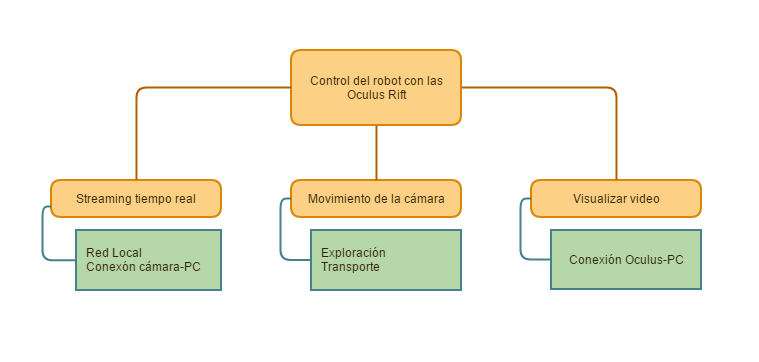
\includegraphics[width=7.00in]{images/objetivos.png}}
	}
	\caption{Resumen de los objetivos del proyecto}
\end{figure}
\newpage
\lsection{Metodolog�a y plan de trabajo}



\newpage \thispagestyle{empty} % P�gina vac�a 

\chapter{Realidad Virtual y rob�tica. Estado del arte}
\label{chap:estadodelarte}

\lsection{Introducci�n}

\lsection{Realidad virtual y salud}
\label{sec:VR y salud}

El uso de realidad virtual est� siendo muy �til en medicina, ya que permite estudiar comportamientos en diferentes situaciones de forma bastante realista.

Un ejemplo de esto es la evaluaci�n del deterioro cognitivo en personas que sufren esclerosis m�ltiple. Para dicha evaluaci�n se requiere una gran cantidad de datos sobre la velocidad de procesamiento de la informaci�n, atenci�n, etc...Esto se consegu�a haciendo m�ltiples test que no siempre eran fieles a la realidad.

Ahora se pueden crear entornos virtuales y estudiar el comportamiento de los usuarios en diversas situaciones de forma que el estudio es m�s realista y eficiente. [ref]


Tambi�n se est� estudiando el uso de programas de rehabilitaci�n para que los pacientes no necesiten trasladarse hasta el hospital.

Uno de los estudios se hizo a personas con hemiparesia, con un software que mostraba por pantalla el movimiento de los pies y les mandaba ejercicios para mejorar su capacidad motora. Los resultados de este estudio mostraron que la herramienta de realidad virtual era efectiva para la rehabilitaci�n y muy �til para los pacientes con dificultades para trasladarse hasta el hospital[ref]





\lsection{Rob�tica y realidad virtual.} 
\label{sec:robotica y VR}
La uni�n de rob�tica y realidad virtual es algo que se lleva haciendo desde hace bastante tiempo.

En el campo de la salud una de las aplicaciones son entrenamientos de cirug�ia. La realidad virtual permite crear un entorno semejante al quir�ofano. El estudiante hace uso de herramientas que simulan los utensilios quir�urgicos y puede hacer una "operaci�on virtual" sin riesgo para ning�un paciente y sin necesidad de gastar recursos o un equipo quir�urgico de apoyo . [ref]

En educaci�n hay varios programas de realidad virtual que hacen el aprendizaje m�s sencillo y completo a los estudiantes. Un ejemplo de esto es la visualizaci�n de brazos rob�ticos para dise�ar correctamente el movimiento.
Es relativamente complejo traducir cada movimiento de las articulaciones del brazo rob�tico en la posici�n finla de �ste. Si estas pruebas se hicieran directamente sobre el robot, ser�a muy sencillo romperlo. Con los programas de realidad virtual se simulan todos los movimientos sin peligro de malgastar recursos. [ref]

Otra aplicaci�n es el control remoto de robots, tanto con software que crea una interfaz virtual para que el usuario obtenga de forma clara toda la informaci�n del robot (bater�a, almacenamiento de datos, posici�n...) [ref NASA xD], como interfaces BCIs.

\lsection{BCIs, EEG y realidad virtual}
\label{sec:BCIs, EEG y realidad virtual}
Las interfaces BCIs (Brain Computer Interfaces) aspiran a que el usuario controle el robot a trav�s de pensamientos, al igual que controlamos nuestro cuerpo.Esta aplicaci�n sigue investig�ndose y se van consiguiendo grandes avances. [ref]??

 


\newpage \thispagestyle{empty} % P�gina vac�a 

\chapter{An�lisis, dise�o y desarrollo}
\label{chap:sistemadesarrollado}
En este cap�tulo se explicar� c�mo se ha enfocado el desarrollo del proyecto.

La primera parte trata del an�lisis del problema. Se explican las diferentes partes en las que he dividido el trabajo para su posterior implementaci�n.
Tambi�n se presenta de forma muy general qu� requisitos b�sicos debe cumplir cada parte.

La secci�n de dise�o explica las herramientas que se han utilizado para implementar cada parte y c�mo funcionan.

Por �ltimo se explica de forma m�s detallada c�mo se ha desarrollado cada parte del problema, qu� dificultades han ido apareciendo y c�mo se han solucionado. Tambi�n explica c�mo se ha realizado la integraci�n para conseguir el proyecto final.

\lsection{An�lisis}
El objetivo de este trabajo es conseguir un robot con una c�mara que transmita video a tiempo real. Este video le llegar� a unas gafas de realidad virtual. El robot se conrolar� con el movimiento de cabeza del usuario.

DIBUJO CHULI DE TODO JUNTO

El proyecto por lo tanto se divide en 3 problemas:
\begin{enumerate}
	\item Construcci�n del robot
	\item Streaming
	\item Control del robot
\end{enumerate}

Vamos a desarrollar cada uno de ellos, identificando qu� funcionalidades b�sicas debe cumplir.

\subsection{Construcci�n del Robot}
	
		El robot debe ser un dispositivo f�cil de controlar , que a su vez act�e como una extensi�n de los ojos del usuario, d�ndole a �ste la sensaci�n de inmersi�n en un espacio real o virtual.
		
		
		Por tanto los requisitos que debe cumplir el robot son los siguientes:
		\begin{itemize}
			\item Permitir grabar video y transmitirlo a tiempo real.
			\item Ser capaz de desplazarse en todas las direcciones
			\item Tener la capacidad de recibir comandos de control a trav�s de una red inal�mbica
			\item Ser capaz de que la c�mara apunte en la misma direcci�n que la cabeza del usuario
		\end{itemize}
	
DIBUJO AMPLIADO ROBOT
		
	\subsection{Streaming}

		Se quiere conseguir la m�xima sensaci�n de inmersi�n para la persona que controla el robot.
		
		Para ello uno de los requisitos principales es que la transmisi�n de video sea  a tiempo real, con la m�nima latencia posible.
		
		Por otra parte el usuario ver� el video con  las Oculus Rift, por lo que la imagen debe estar desdoblada (formato SBS, que se eplicar� en la secci�n de desarrollo).

		La transmisi�n debe ser inal�mbrica ya que queremos que el robot tenga total libretad de movimiento, siendo �ste independiente del ordenador.
		
		Dado que la placa que utilizamos en el el robot es la Raspberry Pi 3 tenemos dos opciones para la transmisi�n inal�mbrica: Bluetooth o red Wifi.
		
	\subsection{Control del Robot}
	
		Como hemos dicho anteriormente, el robot pretende ser una extensi�n de los ojos de usuario, por lo que es l�gico que se controle con el movimiento de cabeza de la persona que est� recibiendo el video.
		
		Dentro del control del robot vamos a diferenciar entre control del movimiento del robot y control de la direcci�n de la c�mara:
		
		\begin{itemize}
			\item Movimiento del robot $\rightarrow$ Debemos dise�ar un sistema intuitivo para mover el robot en todas las direcciones con movimientos de la cabeza.
			\item Movimiento de la c�mara $\rightarrow$ la c�mara debe estar apuntando siempre en la misma direcci�n que la cabeza.
			
			Si el usuario mueve la cabeza hacia la derecha o hacia la izquierda, el robot se mover� en esa direcci�n, por lo que no hay que preocuparse por la c�mara.
			
			Para controlar los movimientos verticales vamos a incorporar un servo unido a la c�mara, de forma que �sta se mueva en funci�n de la posici�n de la Oculus. 
		\end{itemize}
		
		
		


\lsection{Dise�o}

	Tras analizar las diferentes funcionalidades del trabajo vamos a ver c�mo est� dise�ado cada componente.
	
	Los principales dispositivos que componen el proyecto son 
	\begin{itemize}
		\item Robot
		\item Router
		\item Oculus Rift
	\end{itemize}
	
	Tambi�n se tratar� el \textbf{dise�o de conexiones} entre los 3 componentes.

	\subsection{Dise�o del robot}
	
	El robot que se utiliza en este proyecto est� basado en un dise�o anterior hecho por (Nombre del alumno que dise�� en robot)
	
	Consta de:
	\begin{itemize}
		\item Una placa base $\rightarrow$ Raspberry Pi 3
		\item Dos ruedas conectadas con dos servos que permiten al robot desplazarse.
		\item Una c�mara Logitech, conectada a la placa por USB
		\item Un servo conectado a la c�mara 
	\end{itemize}
	
	
	FOTO ROBOT
	
	\subsubsection{Raspberry Pi 3 model B}
	
	La Raspberry Pi 3 model B es un ordenador de placa reducida que lleva un sistema operativo Linux.
	
	Su procesador es un ARM Cortex A53 de cuatro n�cleos a 1.2GHz de 64 bits.
	
	Tiene 1 GB de memoria RAM , 4 puerto USB, 40 pins GPIO, puerto HDMI , Ethernet y entrada para MicroSD.
	
	Adem�s tiene Wifi 802.11n integrado y bluetooth 4.1.
	
	
	\begin{figure}[h]
		\centerline{
			\mbox{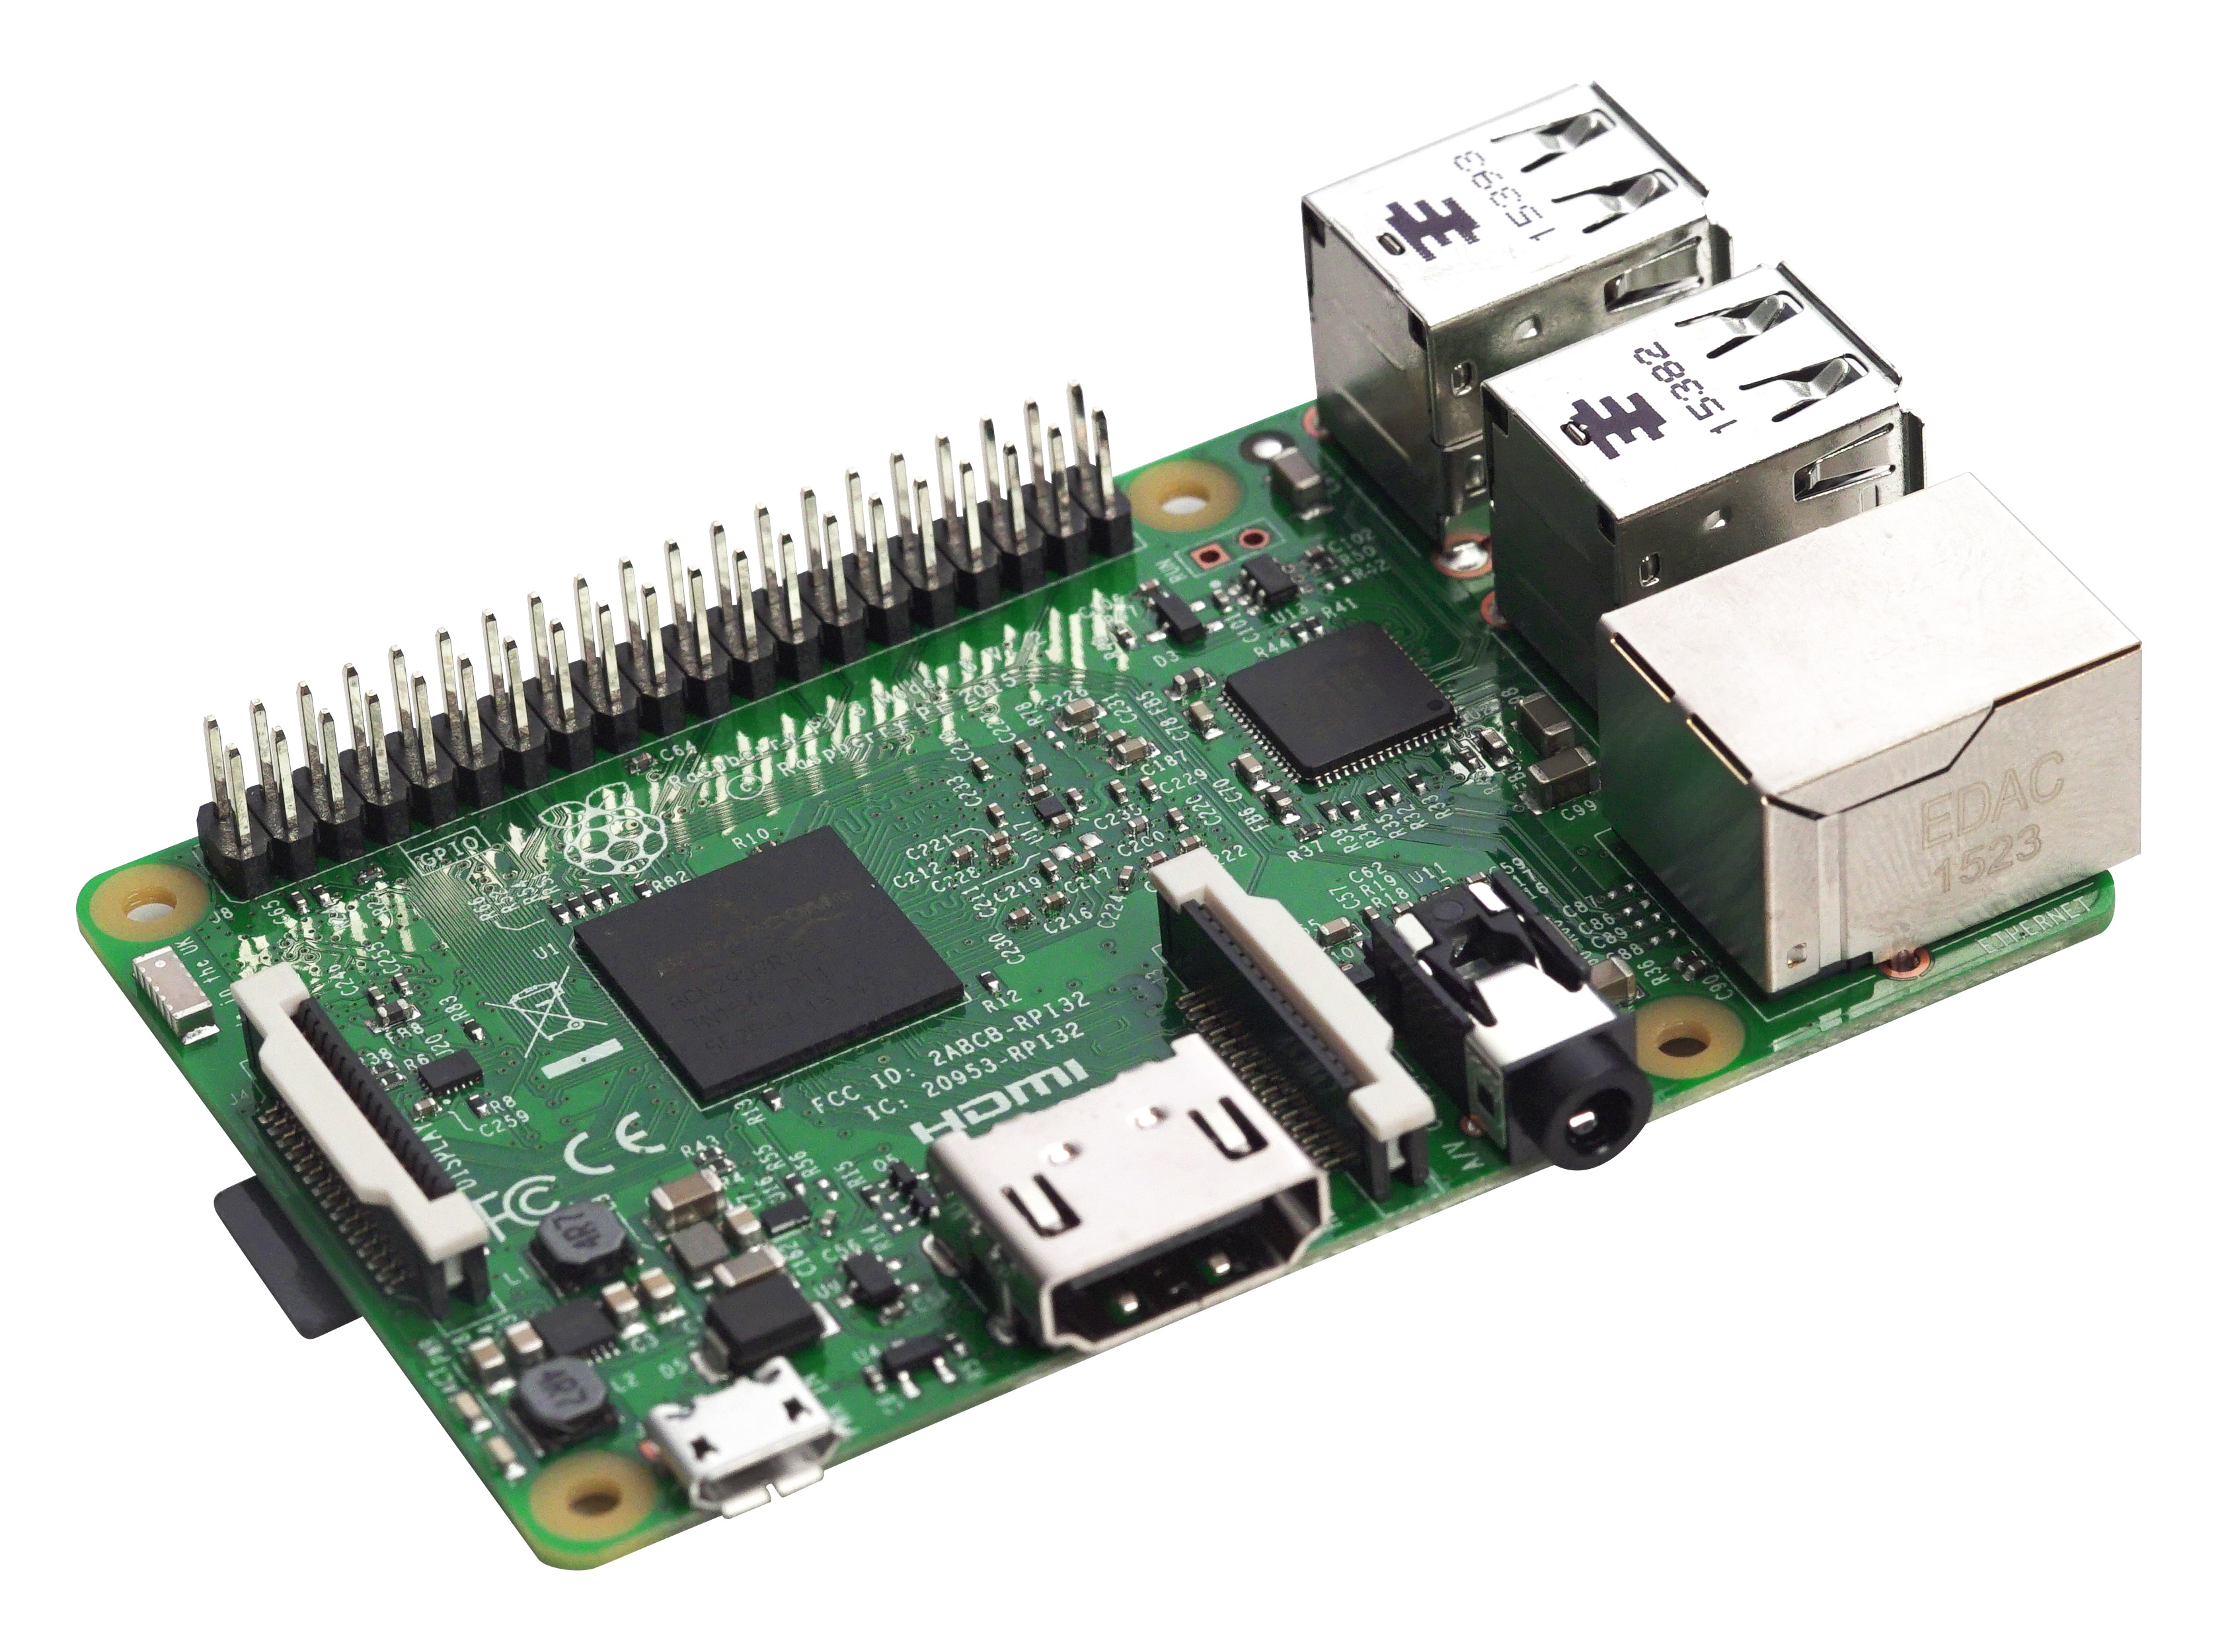
\includegraphics[width=3.00in]{images/raspi3.jpg}}
		}
		\caption{Raspberry Pi 3 model B}
		
	\end{figure}

\subsubsection{Servo motores}
Para el movimiento del robot y de la c�mara utilizamos servo motores


Un servo motor es un motor el�ctrico que se puede controlar su velocidad y su posici�n (dentro del rango de posici�n permitido).

Los servos constan de:
\begin{itemize}
	\item Un motor de corriente continua
	\item Una caja reductora
	\item Un circuito de control
\end{itemize}

El sistema que utilizamos para controlar la velocidad y la posici�n de los servos es la modulaci�n por anchura de pulso (PWM).

\paragraph{PWM}

Este sistema consiste en generar una onda cuadrada en la que se var�a el tiempo que el pulso est� a nivel alto, manteniendo el mismo per�odo (normalmente), con el objetivo de modificar la posici�n del servo seg�n se desee.

\begin{figure}[h]
	\centerline{
		\mbox{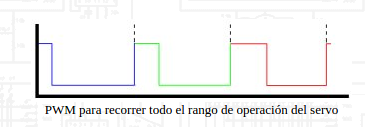
\includegraphics[width=3.00in]{images/ondaServo.png}}
	}
	
\end{figure}



Para que un servo se mantenga en la misma posici�n durante un cierto tiempo, es necesario enviarle continuamente el pulso correspondiente.


La otra funci�n del PWM hemos diche que era el control de velocidad.

Esto lo hace alimentando el motor con una se�al de pulsos con la frecuencia suficiente para que el motor no note las variaciones y haga un giro constante, ya que variando el porcentaje de tiempo de la se�al rectangular en alta, y en baja, variamos la potencia que le entregamos al motor, con lo que controlamos la velocidad de giro con mucha precisi�n.

En el robot utilizamos 3 servomotores.
Dos de ellos se utilizan para el movimiento de las ruedas y el tercero mover� la c�mara permitiendo al usuario mirar hacia arriba y hacia abajo.

Los tres servos est�n controlados por el movimiento de la cabeza del usuario, que obtenemos gracias a las Oculus Rift.

\subsubsection{C�mara}

La c�mara utilizada es una webcam USB. El proyecto tambi�n se podr�a haber hecho con una RaspiCam.

A continuaci�n se muestra un esquema de la conexi�n entre los componentes que acabamos de explicar.


\begin{figure}[h]
	\centerline{
		\mbox{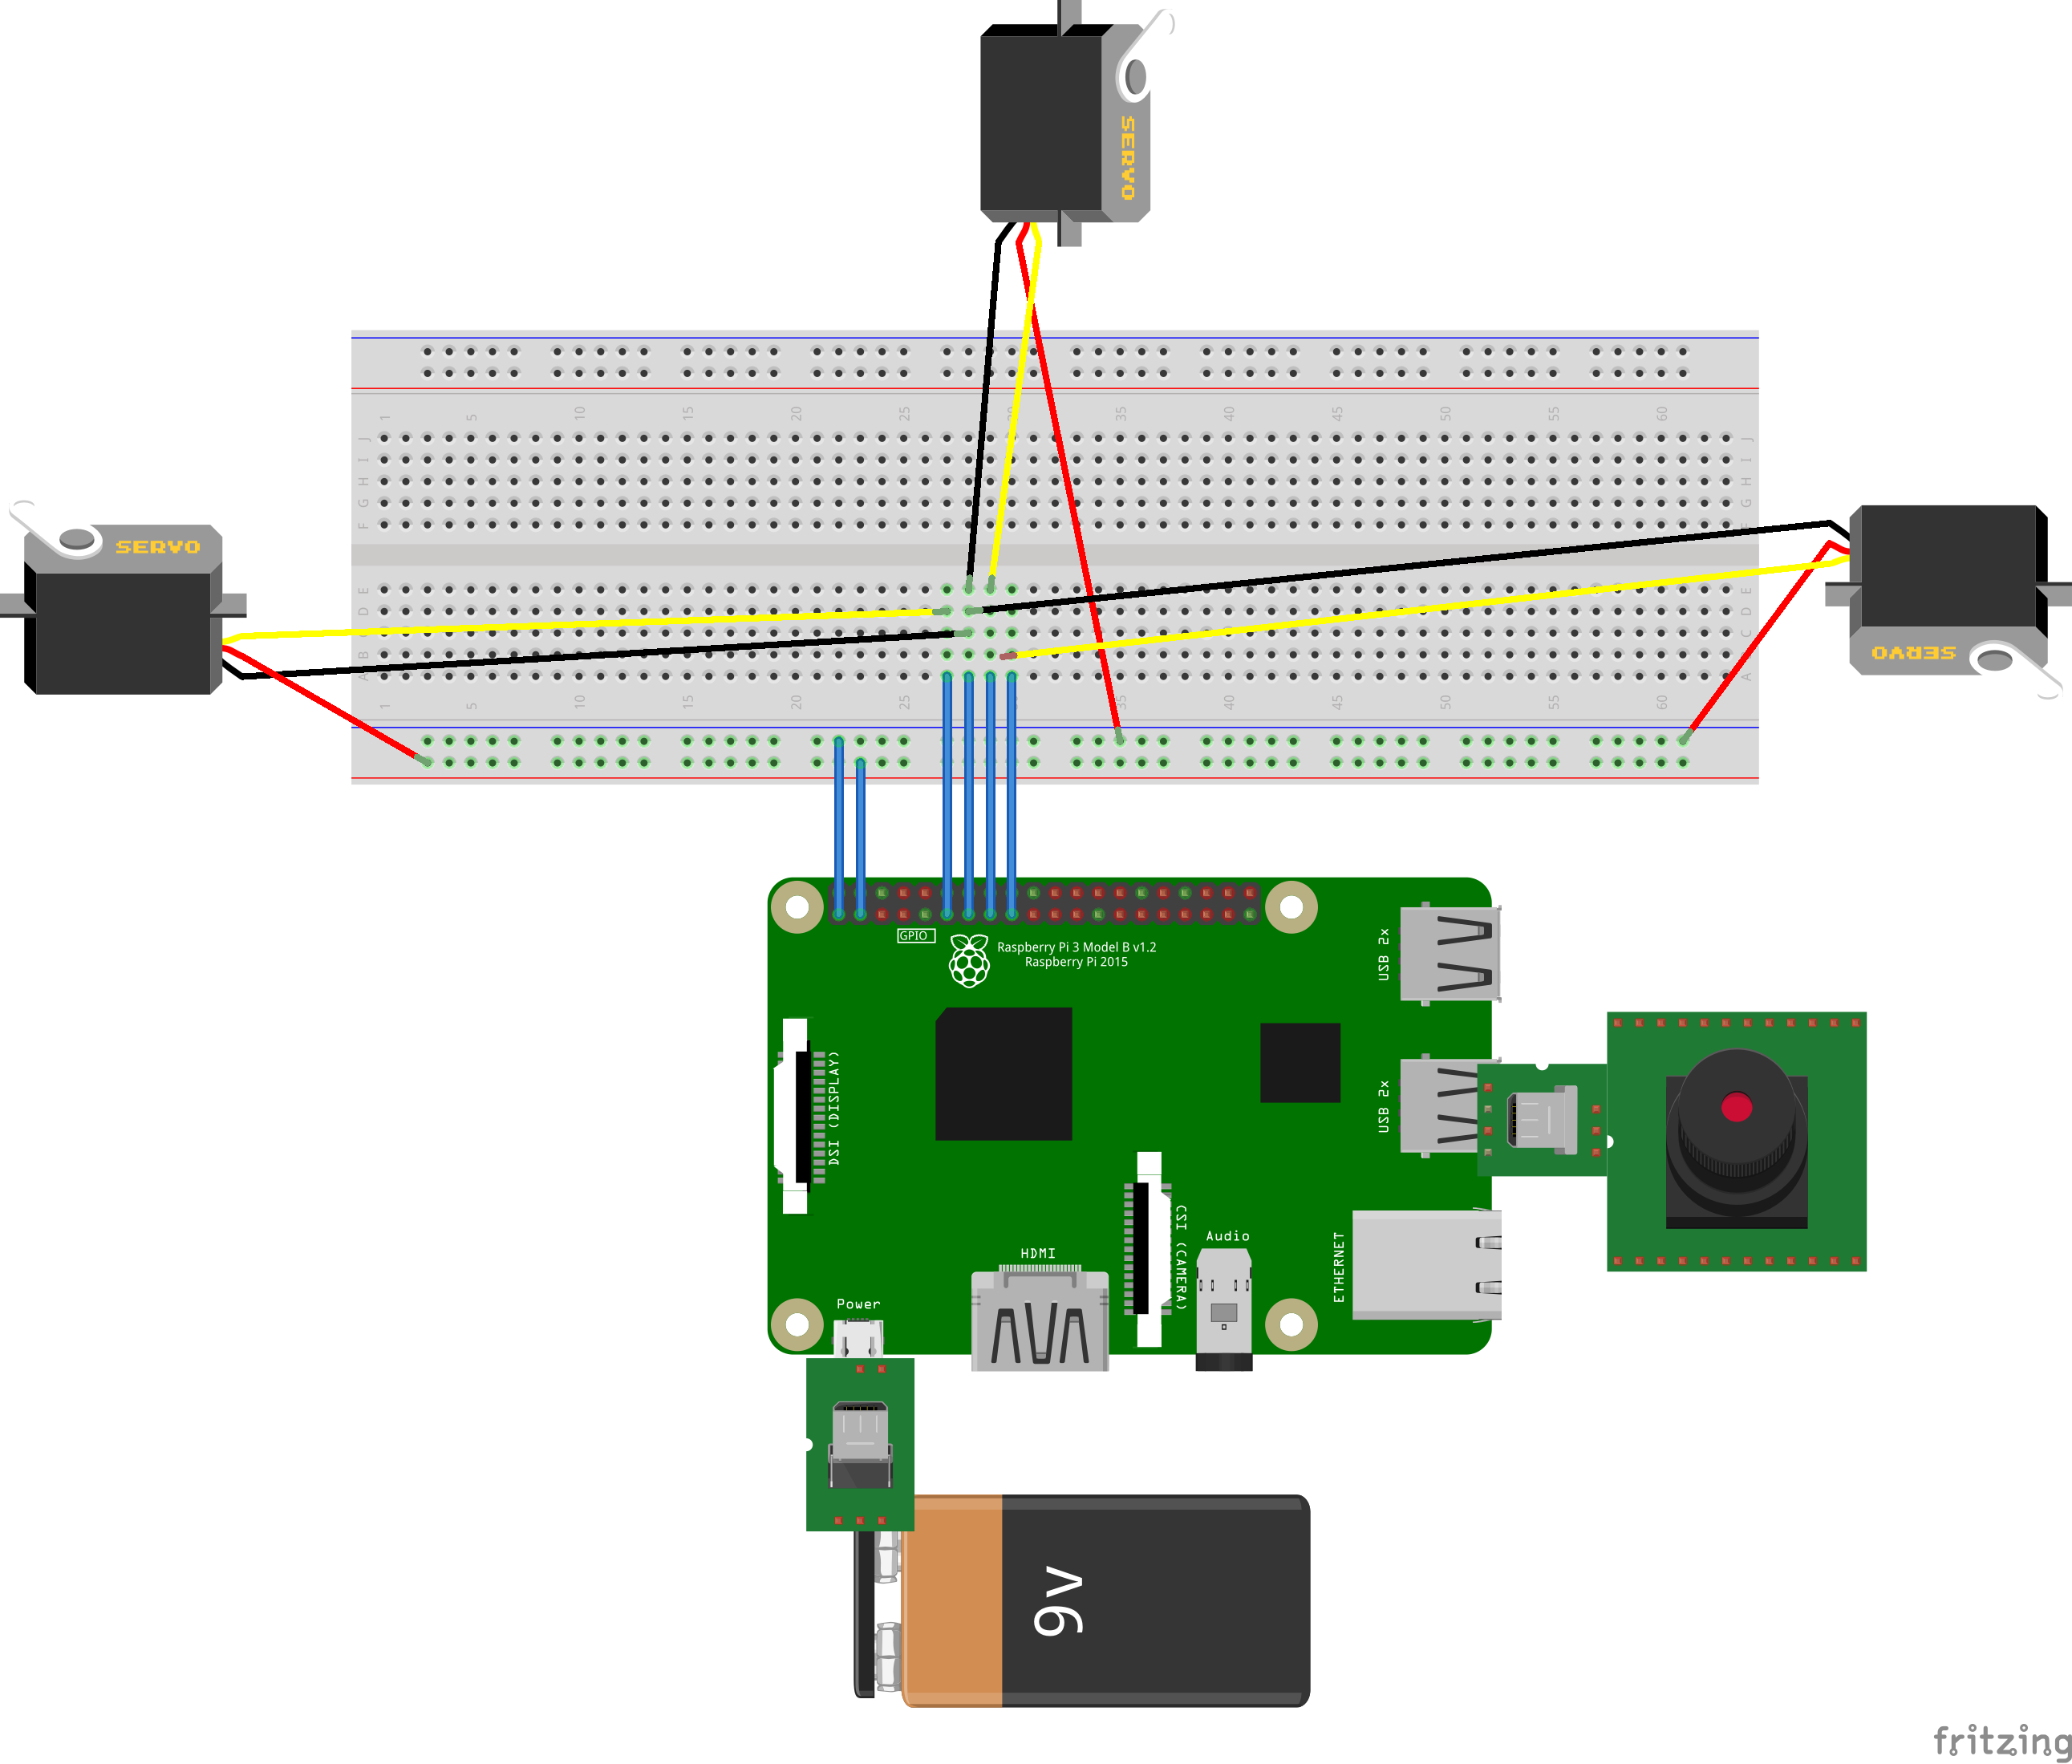
\includegraphics[width=3.00in]{images/EsquemaServos.png}}
	}
	\caption{Esquema conexiones servos , c�mara, Raspberry Pi 3}
\end{figure}


\subsection{Router}
\subsection{Oculus Rift}

Las Oculus Rift son unas gafas de Realidad Virtual [parrafo definiendo las Oculus]

De las gafas nos interesan especialmente:
\begin{itemize}
	\item Detecci�n de la orientaci�n de las Oculus
	\item Recepci�n de video
\end{itemize}

\subsubsection{Detecci�n de la orientaci�n}



Las Oculus Rift tienen integradas un giroscopio, un aceler�metro y un magnet�metro que manda constantemente informaci�n al ordenador, de forma que �ste sabe en todo momento la orientaci�n de las gafas.

La t�cnoca para interpretar la se�al de estos sensores se llama \textbf{fusi�n de sensores}

A continuaci�n se explica en qu� consiste esta t�cnica.

\paragraph{Fusi�n de Sensores }

Como ya hemos mencionado, en las Oculus tenemos un giroscopio, un aceler�metro y un magnet�metro.

Los dos primeros dan informaci�n acerca de la orientaci�n respecto a los ejes X y Z, mientras que el magnet�metro mide la orientaci�n respect al eje Y.

Vamos a ver c�mo funciona cada uno.

El \textbf{giroscopio} de las Oculus mide el cambio de orientaci�n de la cabeza a una velocidad de 1KHz.

Una forma simplificada de calcular la orientaci�n actual es:

$$\text{Orientaci�n actual } = \text{ Orientaci�n anterior } + \text{ Diferencia horaria } \cdot \text{ Velocidad observada (giroscopio).}$$

El problema est� en que la cabeza puede rotar alrededor de tres ejes.

\begin{figure}[h]
	\centerline{
		\mbox{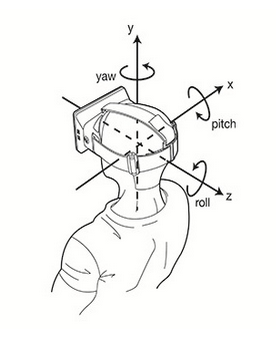
\includegraphics[width=3.00in]{images/headtracking.png}}
	}
	\caption{Ejes de giro}
\end{figure}

Vamos a suponer que solo rotase alrededor del eje Y y que el sensor captase una velocidad angular $w$ por segundo.

Si tuvi�ramos 1000 sensores la f�rmula de la orientaci�n ser�a:

$$\text{Orientaci�n actual } = \text{ Orientaci�n anterior } + 0,001 \cdot w$$

Pero en el caso de las Oculus, al estar midiendo un objeto que se mueve en 3 ejes, el giroscopio da la velocidad angular respecto de los tres ejes, devolviendo un vector 3D ($w_1,w_2,w_3$)

Al basar nuestro c�lculo en el c�lculo anterior, el error ir� creciendo con el tiempo.

Vamos a llamar \textit{tilt error} al error en la medici�n de los �ngulos sobre los ejes XZ. El error sobre el eje Y se llamar� \textit{yaw error}.

El \textit{tilt error} se corresponde con nuestra sensaci�n de lo que "est� arriba", percepci�n que se basa en la gravedad.

La gravedad se expresa con un vector de aceleraci�n , por lo que utilizamos un \textbf{aceler�metro} para medirla.

Nos encontramos con el inconveniente de que el aceler�metro no solo mide la gravedad. Para asegurarnos de que el momento en el que tomamos los datos de referencia solo estamos midiendo la gravedad, esperamos a que se den 2 condiciones:
\begin{enumerate}
	\item El aceler�metro nos devuelve una medida cercana a 9,8
	\item El giroscopio nos devuelve una velocidad angular muy lenta (es decir, no estamos girando).
\end{enumerate}

En este momento sabemos que nos encontramos en una posici�n vertical y podemos corregir el error.

\textbf{C�mo corregimos el error:}
Supongamos que se dan las dos condiciones previas, y la posici�n que nuestro c�lculo de orientaci�n nos devuelve un vector $\vec{a}$, tal y como vemos en el dibujo.

Tenemos el �ngulo $\theta$ entre el eje Y y el vector $\vec{a}$ pero �c�mo calculamos el eje de rotaci�n para rotar $\vec{a}$ y corregir el error?

Dicho vector debe ser perpendicular a $\vec{a}$ y al eje Y, y apoyarse en el plano XZ.

Para encontrar el vector basta con hacer la proyecci�n de $\vec{a}$ en el plano XZ, obteniendo as� ($a_x, 0 , a_z$). Haciendo un vector perpendicular a �ste obtenemos ($-a_z, 0 , a_x$). Y ya tenemos el eje de rotaci�n que necesitabamos para corregir el error.

\begin{figure}[h]
	\centerline{
		\mbox{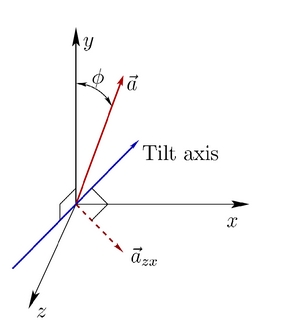
\includegraphics[width=3.00in]{images/ejestracking.png}}
	}
	\caption{Correcci�n del tilt error}
\end{figure}


\newpage
\textbf{Error sobre el eje Y (yaw error)}

Este error se basa en nuestra percepci�n de d�nde est� el norte.

Para esto utilizamos el magnet�metro. COMPLETAR

\subsection{Dise�o de conexiones}

La arquitectura del proyecto es muy sencilla, como podemos observar en la siguiente imagen:

\begin{figure}[h]
	\centerline{
		\mbox{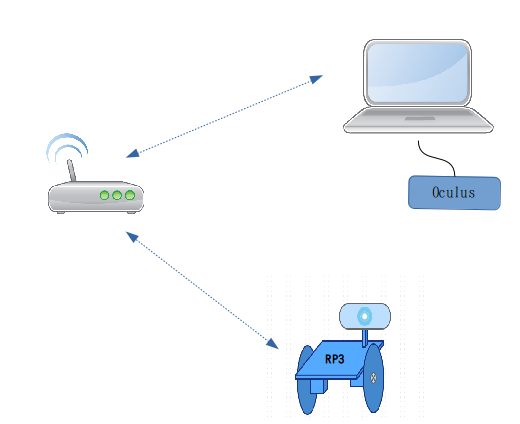
\includegraphics[width=3.00in]{images/EsquemaConexiones.png}}
	}
	\caption{Esquema conexiones}
\end{figure}


Como podemos ver en el esquema, las Oculus Rift est�n conectadas al ordenador, el ordenador y la Raspberry se mandan informaci�n a trav�s de un router que crea una red local.

La raspberry recibe en streaming de la c�mara y lo va mandando a una IP disponible dentro de la red local, la (192.168.1.35). A su vez el ordenador accede a esa IP, recoge el streaming utiliza VLC para dividir la imagen (SBS) y reproducir el video y con la herramienta Virtual Desktop podemos ver el video desde las Oculus.

Por otra parte las Oculus tienen integrado un giroscopio , un aceler�metro y un magnet�metro.

Combinando la informaci�n de estos sensores a trav�s de un proceso conocido como fusi�n de sensores se determina la orientaci�n de la cabeza del usuario en el mundo real , y se sincroniza con la perspectiva virtual del usuario en tiempo real. 

Se ha implementado un programa en phyton que recoge esa informaci�n y la traduce en comandos sencillos para mandarselos a la Raspberry. Para obtener esa informaci�n hacemos uso de la librer�a de las Oculus (ovr).

La Raspberry lee los comandos del ordenador y mueve los servos seg�n lo recibido, de esta forma controlamos el movimiento del robot y de a c�mara.

\newpage
\lsection{Desarrollo e implementaci�n}
En esta secci�n se explicar� c�mo hemos desarrollado las distintas funcionalidades del proyecto.
Para ello vamos a diferenciar entre:

\begin{itemize}
	\item Construcci�n del Robot
	\item Streaming 
	\item Control del Robot
\end{itemize}

Para conseguir \textbf{transmitir a las Oculus el video en tiempo real} es necesario que:
\begin{enumerate}
	\item La Raspberry recoja el video de la c�mara y lo transmita al ordenador.
	
	\item El ordenador recoja el video, lo transforme a formato SBS y lo env�e a las Oculus Rift. 
	
\end{enumerate}

		



Para el \textbf{control del robot} se deber�n implementar las siguientes tareas:

\begin{enumerate}
	\item Leer la se�al de los sensores de las Oculus Rift (giroscopio, aceler�metro y magnet�metro) para saber la orientaci�n de la cabeza del usuario.
	
	\item Transmitir la informaci�n obtenida al robot.
	
	\item Traducir dicha informaci�n en comandos para mover los servo motores.
\end{enumerate} 

\subsection{Streaming}
\subsubsection{Raspberry Pi3}
El primer elemento en el streaming de video es la Raspberry Pi, que tiene conectada por usb una c�mara.

Para recoger el video y mandarlo en tiempo real utilizamos la librer�a mjpeg-streamer, disponible en github.

Mjpeg-streamer es una aplicaci�n en linea de comandos que permite crear un servidor, para retransmitir im�genes JPG sobre una red basada en IP, desde la c�mara hasta un navegador convencional.

Soporta la compresi�n por hardware (GPU, Unidad de Procesamiento Gr�fico) de la c�mara, en nuestro caso H.264 Advanced Video Coding (AVC) Standard, que es el compreso de la Webcam Logitech.

Esto permite reducir dr�sticamente el uso de la CPU de este servidor, haciendo est� aplicaci�n un servicio ligero.

El puerto que emplea es el 8080

\begin{figure}[h!]
	\centerline{
		\mbox{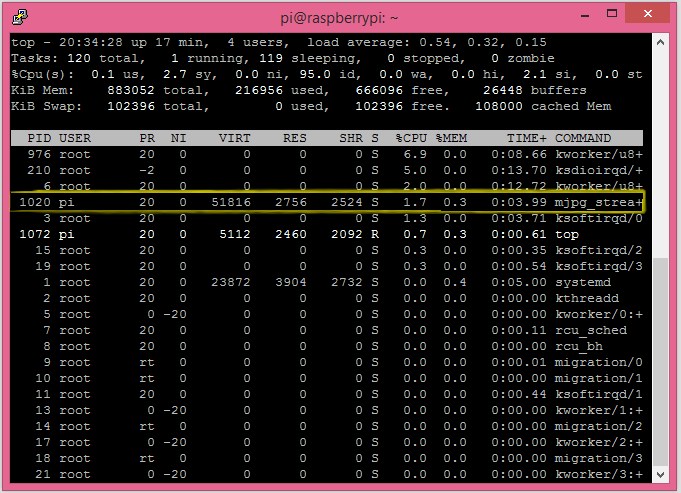
\includegraphics[width=3.00in]{images/UsoCPUMjpeg.png}}
	}
	\caption{Uso de CPU del programa Mjpeg-Streamer por el que se hae el streaming de video}
\end{figure}


\newpage
\subsubsection{Ordenador}
El ordenador accede a la IP donde mjpeg-streamer est� retransmitiendo el video y lo recoge a trav�s del reproductor de video VLC.

Este reproductor divide el video en dos pantallas exactamente iguales para poder verlo desde las Oculus en modo SBS (Side by Side).

El ordenador tiene instalado un programa, Virtual Desktop.

Virtual Desktop es una aplicaci�n desarrollada por Oculus Rift y  HTC Vive para utilizar las Oculus Rift en Windows.

Permite ver el escritorio desde las Oculus, pudiendo configurar efectos como ver las imag�nes SBS o cambiar el entorno en el que te encuentras (el espacio, una sala de cine...)


\begin{figure}[h]
	\centerline{
		\mbox{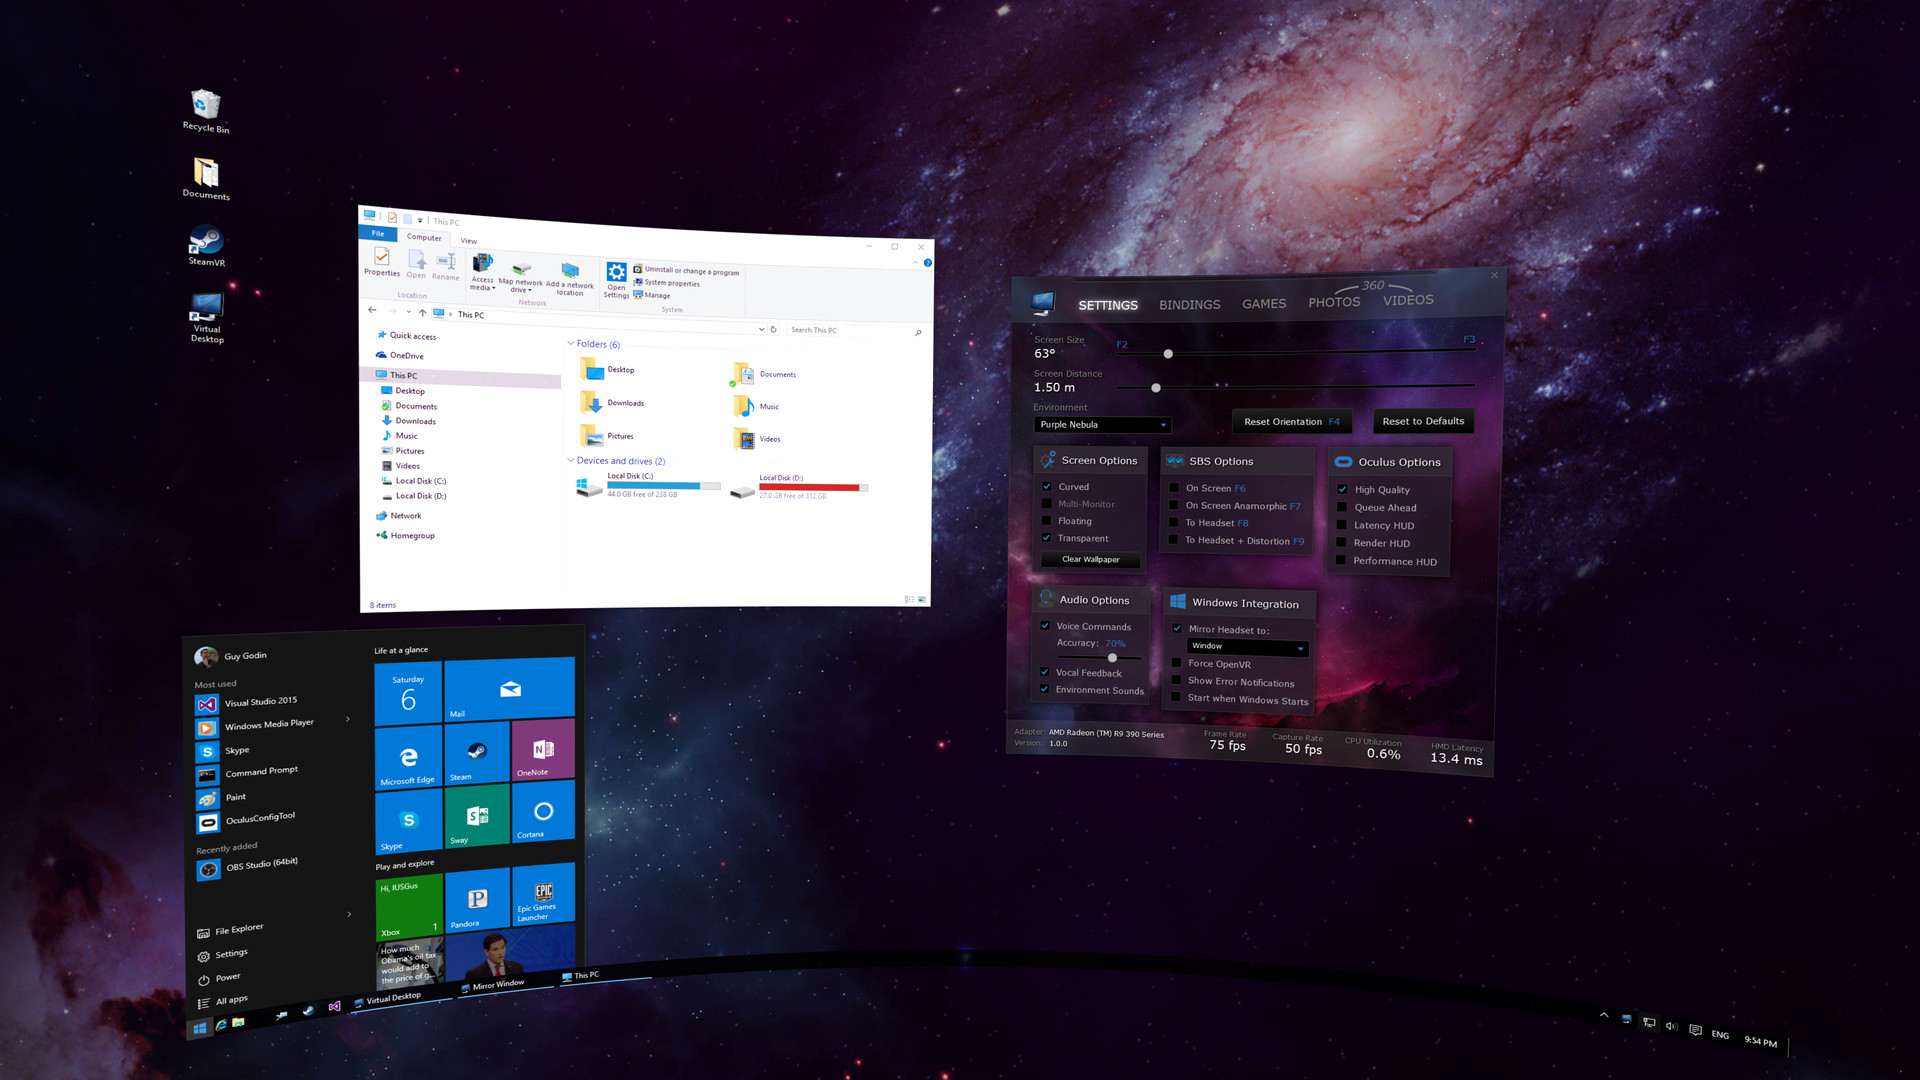
\includegraphics[width=3.00in]{images/VirtualDesktop.jpg}}
	}
	\caption{Virtual Desktop}
\end{figure}

Tambi�n te permite ver videos descargados en el ordenador y reproducir videos 360.

Nosotros utilizamos la funcionalidad de ver la pantalla del ordenador desde las Oculus con SBS, para visualizar el video que se est� reproduciendo en VLC a tiempo real.


IMAGEN DEL VIDEO SBS DE VLC




\subsection{Control del Robot}


\subsubsection{Librer�a OVR}
Para recoger desde el ordenador la informaci�n que mandan las Oculus utilizamos la librer�a de Oculus (ovr), escrita en phyton.

La funci�n \textit{ovr.getTrackingState} nos devuelve una estructura (\textit{TrackingState}), que contiene el campo:

	 \textbf{Pose Statef} HeadPose 
	\begin{itemize}
		\item \textbf{Posef} ThePose $\begin{cases}
			 \textbf{Quatf} \text{ Orientation}\\
			 \textbf{Vector3f}\text{ Position} 
		\end{cases}$
		

	\end{itemize}

Para obtener la orientaci�n de la cabeza se lee el valor de \textit{HeadPose.ThePose.Orientation.x/y} y se lo manda a la raspberry a trav�s de sockets.

La informaci�n obtenida sobre la orientaci�n respecto al eje $x$ servir� para mover los servos que hay en las ruedas del robot, mientras que la informaci�n de $y$ servir� para mover la c�mara.


El ordenador crea un servidor y abre dos sockets distintos, uno para la informaci�n de $x$ y otro para la de $y$.
  

De esta forma manejamos los dos movimientos de forma independiente.

A continuaci�n se muestra una gr�fica que compara el movimiento (en grados) de las Oculus y de un servo motor respecto al tiempo , medido en microsegundos.

Vemos que la latencia entre la medici�n en las Oculus y la recepci�n en la Raspberry es muy peque�a.

\begin{figure}[h!]
	\centerline{
		\mbox{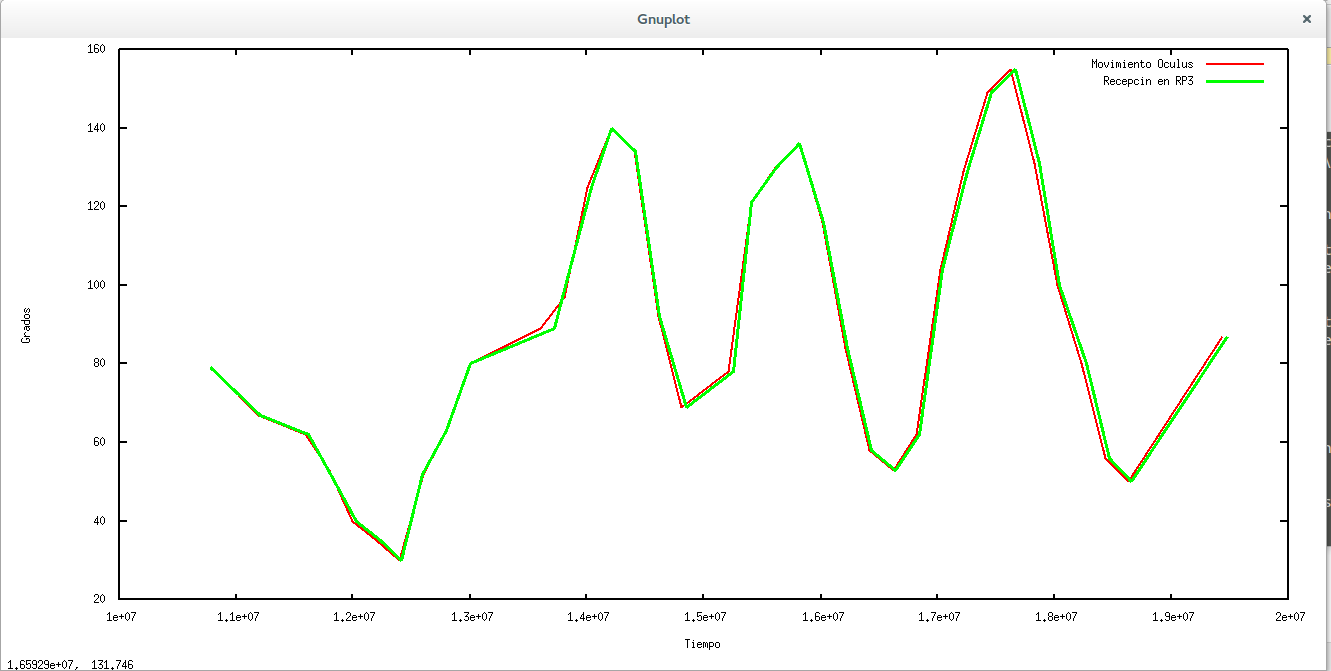
\includegraphics[width=3.00in]{images/TiemposRecepcion(us).png}}
	}
	\caption{Virtual Desktop}
\end{figure}

\newpage
\subsubsection{Raspberry Pi3}
La Raspberry tiene a su vez dos programas (uno para las ruedas y otro para la c�mara) que est�n escuchando continuamente lo que manda el ordenador y en cuanto recibe el comando lo manda a los servos.

\paragraph{Movimiento de los servo motores}

Como ya se indic� en la secci�n (seccion de los servos,PWM, etc..) el movimiento de los servos se controla con una se�al PWM (Pulse With Modulation).

Por ello utilizamos la librer�a RPi.GPIO, que ofrece funciones para PWM.

Hay dos par�metros principales para determinar el pulso que se env�a al motor:
\begin{itemize}
	\item \textbf{Frecuencia} : veces por segundo que se genera el pulso.
	\item \textbf{Duty cycle} : es el porcentaje de tiempo que el pulso est� arriba. (recordemos que la se�al es una se�al cuadrada)
\end{itemize}


Veamos un ejemplo para clarificar esto:

\paragraph{PWM- Frecuencia:50Hz , DutyCycle $50\%$}
	
		
	
	 Si fijamos una frecuencia de 50Hz estaremos mandando una se�al de 50 pulsos por segundo, es decir, un pulso cada $0.02$ segundos.
	
	Al poner un DutyCycle al $50\%$ estamos estableciendo que durante esos $0.02$ segundos el pulso estar� $0.01$ segundos en posici�n "High" y el resto del tiempo en posici�n "Low".
	
	
	\paragraph {PWM- Frecuencia:50Hz , DutyCycle $80\%$}
		
	Si fijamos una frecuencia de 50Hz, como la del ejercicio anterior pero por el contrario ponemos un DutyCycle del $80\%$ tendremos:
	\begin{itemize}
		\item 1 pulso cada $0.02$ segundos
		\item El pulso estar� en posici�n "high" el $80\%$ del tiempo ($0.016$ segundos) y en posici�n "low" los otros $0.004$ segundos restantes.
	\end{itemize}



La Raspberry Pi recibe a trav�s de los sockets el �ngulo de orientaci�n de la cabeza sobre el eje y o x.

Para transformar este �ngulo el pulso(PWM) correspondiente debemos tener en cuenta que un servo requiere una se�al PWM con un periodo de 20 ms y un ancho de pulso entre $0.9$ y $2.1$ ms.

Ya que el servo tiene un rango de �ngulos de 0 a 180 grados, es f�cil ver que el ancho de pulso de $0.9$ ms se corresponde con 0� y $2.1$ ms con 180�







\lsection{Segmentaci�n}

\lsection{Normalizaci�n}

\lsection{Codificaci�n}

\lsection{Matching}


\chapter{Experimentos Realizados y Resultados}
\label{chap:experimentos}

\lsection{Bases de datos y protocolo}

\lsection{Sistemas de referencia}
\label{sect:sistemasreferencia}

\lsection{Escenarios de pruebas}
\label{sect:escenarios_pruebas}
 
\lsection{Experimentos del sistema completo}


\chapter{Conclusiones y trabajo futuro}
\label{chap:conclusiones}
\vspace{-0.2cm}

\lsection{Conclusiones}
Tras realizar el trabajo y probarlo con numerosas personas, concluyo que es un proyecto con una muy buena acogida, f�cil de desarrollar con las herramientas de las que disponemos y con mucho potencial, ya que incluye dos tecnolog�as que est�n en pleno desarrollo y que a�n tienen mucho que avanzar.

Otra ventaja es que hace uso de dispositivos de f�cil acceso por lo que no resultar�a demasiado caro de fabricar.

 

\lsection{Trabajo futuro}
Este trabajo es solo el inicio de lo que podr�a ser un proyecto muy interesante.

El robot que hemos construido es una extensi�n del sentido de la vista, pero se podr�a construir un robot controlado por una persona y que fuera la extensi�n de todos sus sentidos,permitiendo as� conocer y sentir el mundo sin necesidad de moverse de su casa.

Adem�s la realidad virtual es una herramienta muy potente, que no solo te permite modificar tu mundo a placer sino que te premita crear entornos totalmente distintos. Se podr�a estudiar c�mo interactuar con ese mundo virtual no solo a trav�s de la vista , sino con todos los sentidos.

Otro camino por el que se puede investigar es la uni�n de este proyecto con la dom�tica.
Creo que en un futuro no muy lejano, las casas ser�n casas domotizadas, que igual que se podr�n controlar desde el m�vil podremos controlass con las gafas de realidad virtual.





\newpage \thispagestyle{empty} % P�gina vac�a 

\chapter*{Glosario de acr�nimos}
\addcontentsline{toc}{chapter}{Glosario de acr�nimos}

\begin{itemize}
\item{\textbf{IS}:  Iris Subject}
\item{\textbf{DCT}: Discrete Cosine Transform}
\item{\textbf{WED}: Weighted Euclidean Distance}

\end{itemize}

\newpage \thispagestyle{empty} % P�gina vac�a

\addcontentsline{toc}{chapter}{Bibliograf�a}    %Agregamos al �ndice el capitulo de bibliograf�a 

\bibliographystyle{unsrt}   %plain pero ordenado en orden de aparacicion en documento principal
\bibliography{bibliografia}

\appendix   %Indicamos que lo que viene a continuaci�n son ap�ndices

%\frontmatter %Para poner los anexos en numeros romanos

\chapter{Manual de utilizaci�n}
\label{Anexo:manualuso}


\newpage \thispagestyle{empty} % P�gina vac�a 

\chapter{Manual del programador}
\label{Anexo:codigosMatlab}


\newpage \thispagestyle{empty} % P�gina vac�a 

%Hoja final en blanco
\newpage \thispagestyle{empty} % P�gina vac�a

\end{document}
